\documentclass[11pt]{article}
%% Package imports
\usepackage[utf8]{inputenc}
\usepackage{amsmath}
\usepackage{subcaption}
\usepackage{amsfonts}
\usepackage{amssymb}
\usepackage{physics}
\usepackage{graphicx}
\usepackage[left=2cm,right=2cm,top=2cm,bottom=2cm]{geometry}
\usepackage{multirow}
\usepackage{booktabs}
\usepackage{float}
\usepackage{verbatim}
\usepackage{amsthm}
\usepackage{minted}
\usepackage{fancyhdr}
\usepackage[shortlabels]{enumitem}
\renewcommand{\baselinestretch}{1.5}

%% Commands for inserting big braces.
\newcommand\lb{\left\lbrace}
\newcommand\rb{\right\rbrace}

%% Commands for set such that notation
\newcommand\st{\text{ } | \text{ }}

%% Math symbols
\newcommand\Q{\mathbb{Q}}
\newcommand\R{\mathbb{R}}
\newcommand\N{\mathbb{N}}
\newcommand\C{\mathbb{C}}
\newcommand\l{\mathcal{l}}

\newtheorem*{theorem}{Theorem}


\parindent 0ex

%% Page style settings
\pagestyle{fancy}
\fancyfoot{}
\fancyhead[L]{\slshape{Formalising Mathematics}}
\fancyhead[R]{\slshape{CID: 01871147}}
\fancyfoot[C]{\thepage}
\begin{document}

\title{Formalising Mathematics - Coursework 1 \\ Intermediate Value Theorem}
\date{\today}
\author{CID: 01871147}
\maketitle

\section*{ Introduction }

In the first part of the coursework I've decided to formalise the intermediate
value theorem which was covered as a part of the course MATH40002: Analysis I
during the first year of my degree. My choice of this theorem was motivated by
the fact that the next two parts of the coursework need to cover concepts that
I've learned in my second and third year of the course respectively. Because of
this, and the fact that as a JMC student I only took one other maths module this
term (which is MATH60029: Functional Analysis), I needed to start building up my
knowledge of formalising proofs in mathematical analysis. \\

This report documents the process of formalising IVT using the Lean programming
language. It is a functional language which can also be used as an interactive
theorem prover. Programming in Lean involves using a wide range of tools, which
given a set of hypotheses allow the programmer to prove a certain statement
(later referred to as the goal). Those tools are called "tactics" in Lean.
These tactics allow the user to perform usual manipulations on the state of the
argument (e.g. introduction of hypotheses). \\

The main advantage of using Lean in order to formalise a theorem is that we can
easily modularise the argument into a set of lemmas which we can then combine
in order to get our desired proof. This is achieved because Lean is a
functional programming language and so the proofs that we formulate are
actually represented as functions which take hypotheses as input and return the
proof of a particular claim a output. That way formulating a proof can in some
cases be thought of as function composition.

\pagebreak

\section*{ Statement of The theorem }

Before we go over the process of formalising the theorem, let us start by
stating it.
\begin{theorem}[Intermediate Value Theorem]
  Let $f : [a, b] \to \R  $ be a continuous function, then for all $c$ between
  $f(a)$ and $f(b)$, there exists $x \in [a, b] $ satisfying $f(x) = c$.
\end{theorem}

In the following sections I will explain the methodology that I used to
formalise the theorem, give its proof and contrast it with the implementation
that I developed in Lean to formalise it.


\section*{ The Process of Formalising }

In order to formalise the theorem I took the following approach. First, I
started by formulating a hand-written proof of the theorem using the course
notes. After I familiarised myself with the argument, I tried to directly
translate it into the Lean code without thinking about the overall structure of
the argument. \\

The interactive theorem proving in Lean works similarly to
compiling a program in any given programming language. The programmer is writing
the code in the editor, while simultaneously the Lean language server protocol
is trying to "compile" the code which effectively checks the validity of the
proof (and incomplete or incorrect proof results in a compilation error).
Consequently, if the proof that we write is correct, then Lean should compile
it without producing any errors.\\

After trying to formalise my argument in one monolithic proof, I eventually
managed to complete it and successfully compile. The main issue I
encountered was that because of the lack of modularity, the proof was very long
and the compilation times were about 5-6 seconds. At some point it started
negatively affecting my experience of using the language, as I couldn't quickly
make adjustments to the proof and see the instant response from the compiler.


\begin{figure}[H]
  \centering
  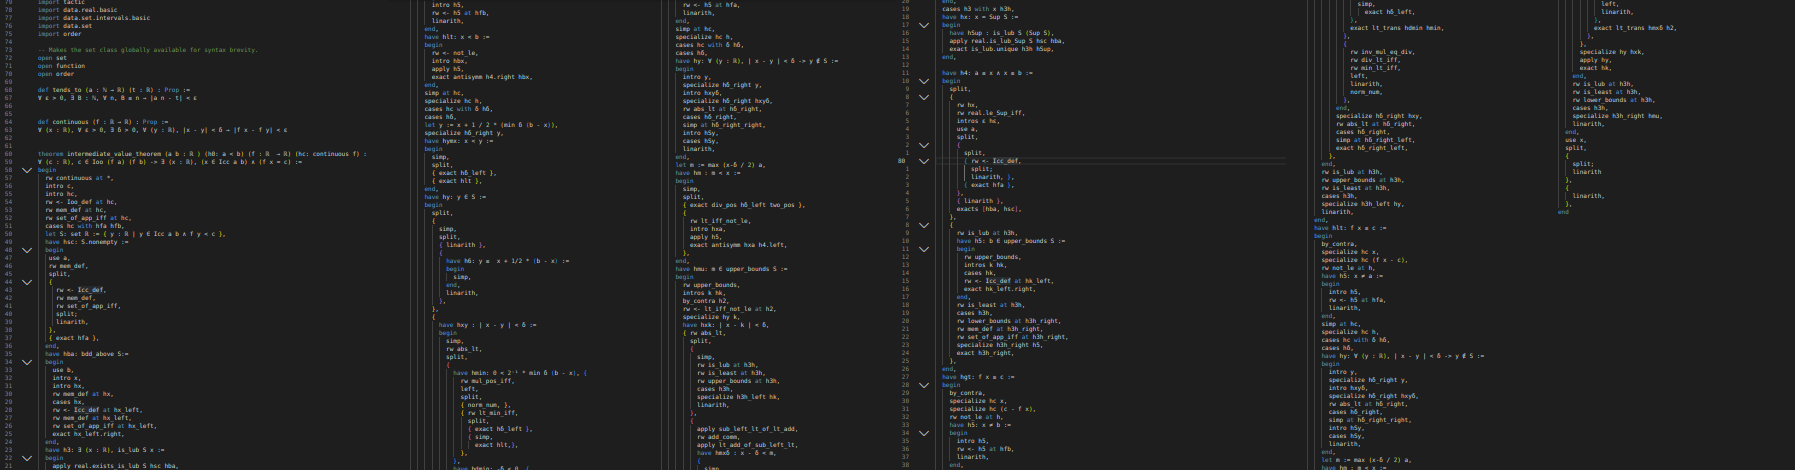
\includegraphics[scale=1.1]{long_code.png}
  \caption{The first inefficient version of the proof}
	\label{long_code}

\end{figure}

In order to solve this issue.

\section*{ Proof of The theorem }


\begin{proof}

\end{proof}
\section*{ Walkthrough in lean }
\section*{ Conclusion }

\end{document}














